\subsubsection{automated}

Splitting the whole computation automately is a good story. Ideally, the whole progress shoule be like the follow picture:

\begin{figure}[ht] 
    \centering  
    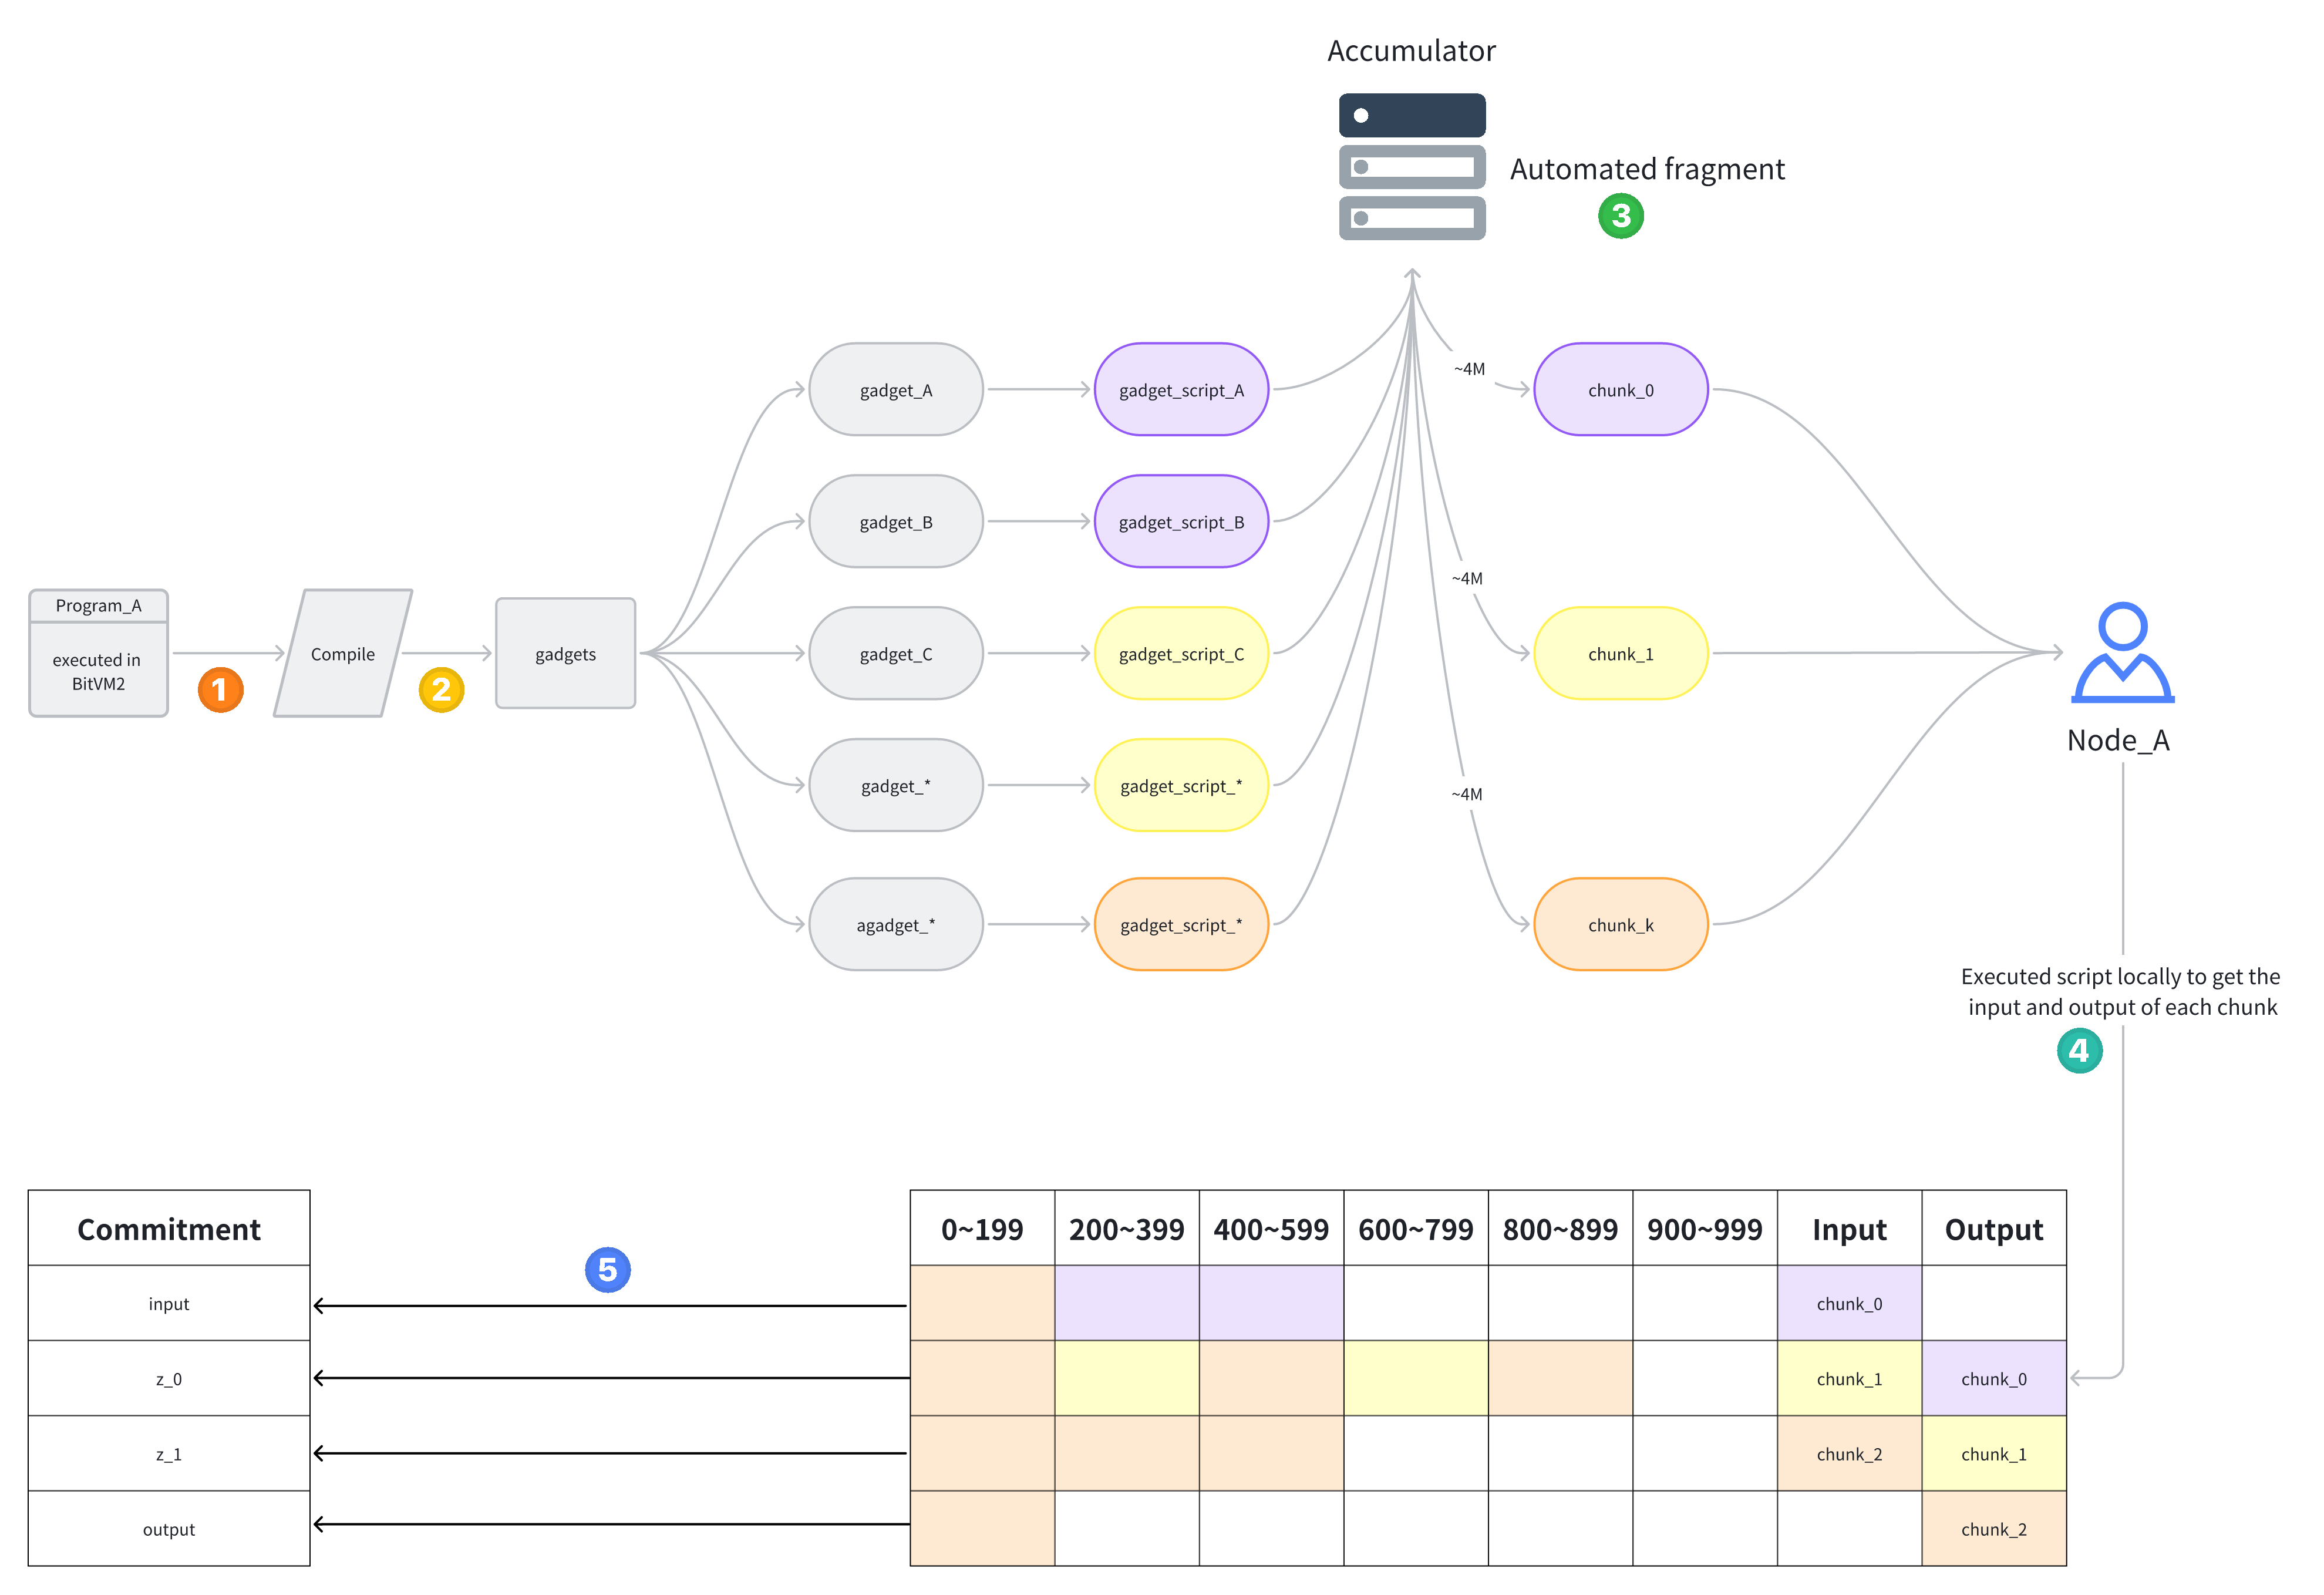
\includegraphics[width=0.85\columnwidth]{images/automated-fragment.png} 
    \caption{automated fragment}
    \label{fig:automated-fragment}
\end{figure}

The overall flow shoule be as follows:
\begin{itemize}
    \item The program will be complied into a set of customized gadgets first
    \item Each gadget will correspond with a script gadget;
    \item The accmulator begin to split the whole gadgets;
    \item Becasue each script gadget has a fixed size, so when the accumulated size is almost equal to 4M, these gadgets will spilt as one chunk;
    \item The Node A execute the script program locally to generates input and output for each chunk;
    \item All the input and output locate in stack, so The Node A have to commit all the value in the stack;
\end{itemize}

It is worth to note that stack depth is another factor shoule be taken into account. For the automated way, we think there have a few constrains:
\begin{itemize}
    \item It is easy to exceed the stack depth limitation;
    \item It committes lot of value which won'be used in current chunk;
    \item It has to implememnt enough gadgets to support any computation which means turing completed;
    \item Executing a big scirpt program is much slow;
    \item It adds the costs when verify the expected input and output on chain;
    \item The logic of each chunk is unreadable;
\end{itemize}

However, automated fragment has some advantages as well, like it will generate the minimal number of script chunk. But as we dont put 
all chunks into Bitcoin network, So we do can not mind the number of chunks unless the size is much big.
